\chapter{Tổng quan}

\section{Giới thiệu về hệ thống robot tự hành thông minh và các ứng dụng}
\subsection{Giới thiệu}

Robotics đã đạt được thành tựu cực kì lớn trong công nghiệp sản xuất với robot công nghiệp như cánh tay robot (manipulator). Cánh tay robot có thể di chuyển với tốc độ và độ chính xác cao, cải thiện đáng kể năng suất và sản phẩm trong sản xuất công nghiệp.
\cite{siegwart2011introduction}

\begin{figure}[h]
    \centering
    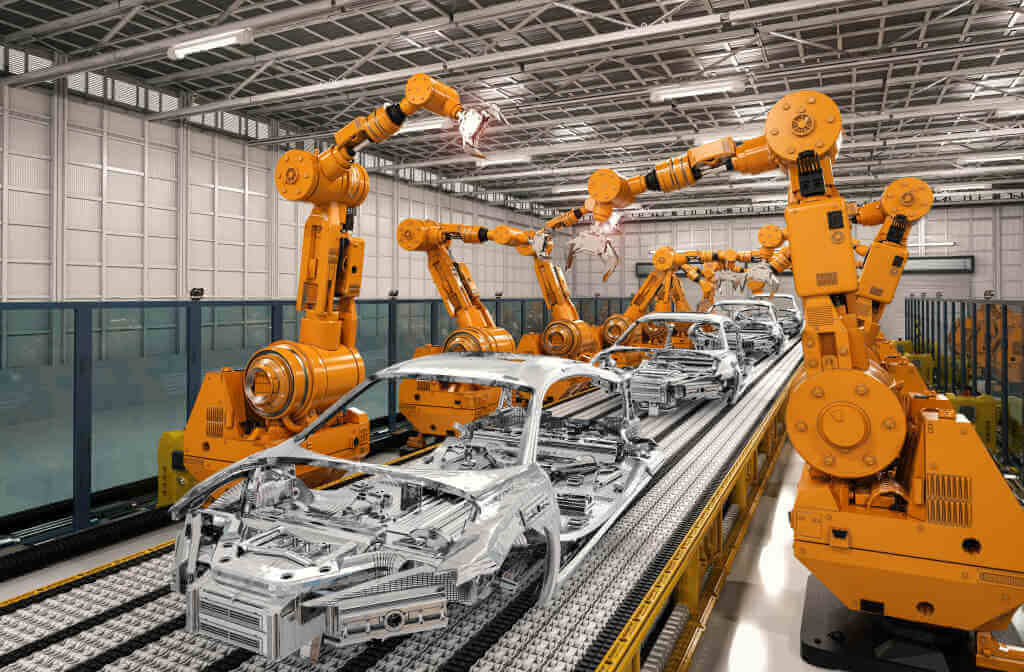
\includegraphics[width=13cm]{chapter1/figs/IndustrialRobot.jpg}
    \caption{Robot công nghiệp}
\end{figure}

Tuy vậy, hạn chế của cánh tay robot là không gian làm việc, bởi vì nó cố định.

Để bổ sung vào hạn chế đó của cánh tay robot công nghiệp, \textit{mobile robot} hay còn gọi là robot di động ra đời. 
Ở thời điểm đầu, mobile robot chỉ có thể làm việc trong giới hạn sự kiểm soát của con người về mặt không gian và hành động. Thông qua việc điều khiển mọi hành động di chuyển của mobile robot. Ví dụ như điều khiển bằng tay thông qua bảng điều khiển, qua sóng RF... hay di chuyển bám line, đọc mã bar, mã QR. Tất cả các phương pháp đó đều khá hạn chế về không gian hoạt động cũng như yêu cầu thiết lập môi trường hết sức tốn kém, kém linh hoạt. Mỗi khi cần thực hiện một nhiệm vụ khác đều phải thiết lập lại nhà máy, không gian làm việc hết sức tốn kém.
Như vậy, làm sao để mobile robot có thể di chuyển trong môi trường thế giới thực mà không cần (hoặc ít) sự kiểm soát, điều khiển của con người để tự nó thực hiện mọi hành động đã đặt ra một số bài toán thách thức cho các nhà nghiên cứu robotics.

Từ đó, robot tự hành thông minh ra đời.

\subsection{Định nghĩa robot tự hành thông minh}
Robot tự hành thông minh là loại robot di động, có thể cảm nhận, mô hình hóa môi trường xung quanh nó. Thực hiện các hành động di chuyển mà không cần sự giám sát cũng như điều khiển trực tiếp từ con người (\figurename{\ref{fig:intro}}).
\begin{figure}
	\centering
	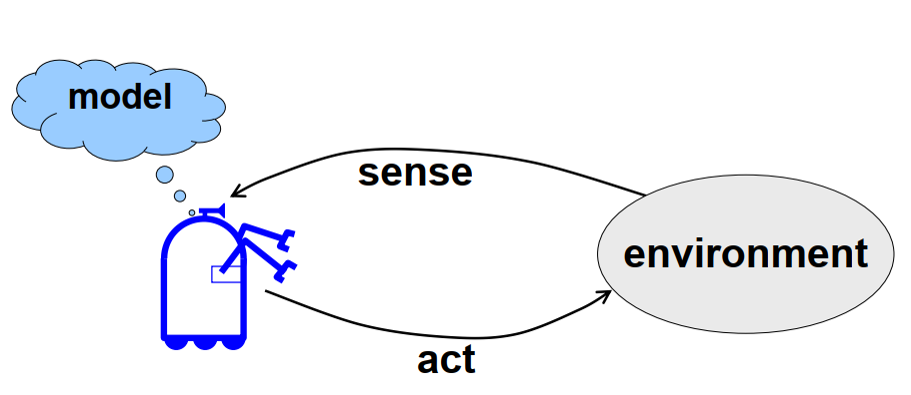
\includegraphics[width=13cm]{chapter1/figs/intro.png}
	\caption{Robot tự hành thông minh}
	\label{fig:intro}
\end{figure}

%\subsection{Phân loại robot tự hành thông minh}

\subsection{Ứng dụng của robot tự hành thông minh}

\section{Các bài toán nghiên cứu trên hệ thống robot tự hành thông minh}

\section{Các nghiên cứu về SLAM}

\section{Sự cần thiết của luận văn}


